\documentclass[12pt]{article}
\usepackage{cwilliams-standard}

\setclass{\URBCOMP}
\settitle{Intro to Urban Computing - Homework 3}

\begin{document}

\maketitlepage

\section{Poor Testing Model}

If a linear regression model is testing poorly, there are two potential reasons that stand out immediately. 

\textbf{Reason 1: Overfitting}. The model could be performing poorly on test data because that model has been trained \textit{too much} on the training data, meaning it has low to no generalizability. The model has taken into account too much training data and is highly sensitive and tries to include it.

\textbf{Reason 2: Underfitting}. The model could also be performing poorly because the model was not trained enough on the training data, meaning that it underfit. It is not taking into account enough of the data to accurately predict, also resulting in low generalizability.

\section{Linear Regression Estimation}

Of the five equations listed, only 2 can be accurately estimated with linear regression. For an equation/function to be estimated accurately 
with linear regression, the function to be \textit{linear in parameters}.

\begin{itemize}
    \item \textbf{a}. $\boxed{y=\sum_{i=0}^{n} a_i x^i}$ is \textbf{estimated accurately}. This is because when it is expanded out into $y = a + a_1 x + a_2 x^2 + a_3 x^3 + ...$, it is linear in parameters and each coefficient only appears once, multiplied by a function of x.
    \item \textbf{b.} $\boxed{y=ax + b \cdot sin(x) + c \cdot \log (x) + d}$ is \textbf{not} estimated accurately. When expanded, terms like $sin(x)log(x)ax$ and $axcd$ appear, meaning the coefficients multiply each other which means that they are not linear, or that the coefficients cannot be separated.
    \item \textbf{c.} $\boxed{y=ae^{(bx)}}$ is \textbf{maybe} estimated accurately. This function could be linearized with log transformations ($\log (y) = \log (a) + bx$) \\
              the parameters are not linear, meaning they cannot be directly estimated with linear regression.
    \item \textbf{d.} $\boxed{y=ax + bx + c}$ is \textbf{estimated accurately}. Since this can simplify to $y = \beta x + c$, where $\beta = (a+b)$, this fits our general form of linear regression, the parameters are linear. We cannot separate the parameters, only find their sum, but that's still pretty good!
    \item \textbf{e.} $\boxed{y = \frac{(ax + b)}{(cx + d)}}$ is \textbf{not} estimated accurately. This does not fit in the general form and the coefficients appear in a non-linear way. And, if this function is plotted (in Desmos), unless $d = 1$, then the function cannot possibly be estimated accurately.
\end{itemize}

\section{Least Squares Methods}

To derive the least squares estimates for a, b, and c, I used the general form of linear regression and then used row reduction to find the least squares.
\begin{equation}
y = ax_1 + bx_2 + c \rightarrow y = X\beta + c \\
\end{equation}

We are trying to find $X^T X$ where $X = [a b c]^T$

\begin{gather}
    X =
    \begin{bmatrix}
        0 & 0 & 1 \\
        0 & 1 & 1 \\
        1 & 0 & 1 \\
        1 & 1 & 1 
    \end{bmatrix} 
    \quad 
    y = 
    \begin{bmatrix}
        0 \\
        1.5 \\
        2.0 \\
        2.5
    \end{bmatrix}
    \quad
    X^T =
    \begin{bmatrix}
        0 & 0 & 1 & 1 \\
        0 & 1 & 0 & 1  \\
        1 & 1 & 1 & 1 
    \end{bmatrix} \\
    X^T X = 
    \begin{bmatrix}
        0 & 0 & 1 & 1 \\
        0 & 1 & 0 & 1  \\
        1 & 1 & 1 & 1 
    \end{bmatrix}
    \begin{bmatrix}
        0 & 0 & 1 \\
        0 & 1 & 1 \\
        1 & 0 & 1 \\
        1 & 1 & 1 
    \end{bmatrix} 
    = 
    \begin{bmatrix}
    2 & 1 & 2 \\
    1 & 2 & 2 \\
    2 & 2 & 4
    \end{bmatrix}\\
    X^T y =
    \begin{bmatrix}
        0 & 0 & 1 & 1 \\
        0 & 1 & 0 & 1  \\
        1 & 1 & 1 & 1 
    \end{bmatrix}
    \begin{bmatrix}
        0 \\
        1.5 \\
        2.0 \\
        2.5
    \end{bmatrix}
    =
    \begin{bmatrix}
        4.5 \\
        4.0 \\
        6.0
    \end{bmatrix}
\end{gather}

Now that we have our necessary equations, we need to solve $(X^TX)\beta = X^Ty$

\begin{gather}
     \begin{bmatrix}
    2 & 1 & 2 \\
    1 & 2 & 2 \\
    2 & 2 & 4
    \end{bmatrix}
    \begin{bmatrix}
        a \\ b \\ c
    \end{bmatrix}
    = 
    \begin{bmatrix}
        4.5 \\
        4.0 \\
        6.0
    \end{bmatrix}
\end{gather}

Original system:
\begin{align}
2a + b + 2c &= 4.5 \tag{1} \\
a + 2b + 2c &= 4.0 \tag{2} \\
2a + 2b + 4c &= 6.0 \tag{3}
\end{align}

Augmented matrix:
\[
\left[\begin{array}{ccc|c}
2 & 1 & 2 & 4.5 \\
1 & 2 & 2 & 4.0 \\
2 & 2 & 4 & 6.0
\end{array}\right]
\]

$R_1 \to \frac{1}{2}R_1$:
\[
\left[\begin{array}{ccc|c}
1 & 0.5 & 1 & 2.25 \\
1 & 2 & 2 & 4.0 \\
2 & 2 & 4 & 6.0
\end{array}\right]
\]

$R_2 \to R_2 - R_1$:
\[
\left[\begin{array}{ccc|c}
1 & 0.5 & 1 & 2.25 \\
0 & 1.5 & 1 & 1.75 \\
2 & 2 & 4 & 6.0
\end{array}\right]
\]

$R_3 \to R_3 - 2R_1$:
\[
\left[\begin{array}{ccc|c}
1 & 0.5 & 1 & 2.25 \\
0 & 1.5 & 1 & 1.75 \\
0 & 1 & 2 & 1.5
\end{array}\right]
\]

$R_2 \to \frac{1}{1.5}R_2$:
\[
\left[\begin{array}{ccc|c}
1 & 0.5 & 1 & 2.25 \\
0 & 1 & \frac{2}{3} & \frac{7}{6} \\
0 & 1 & 2 & 1.5
\end{array}\right]
\]

$R_3 \to R_3 - R_2$:
\[
\left[\begin{array}{ccc|c}
1 & 0.5 & 1 & 2.25 \\
0 & 1 & \frac{2}{3} & \frac{7}{6} \\
0 & 0 & \frac{4}{3} & \frac{1}{3}
\end{array}\right]
\]

From the last row: $\frac{4}{3}c = \frac{1}{3}$, so $c = \frac{1}{4} = 0.25$

Back substitution into row 2: $b + \frac{2}{3}(0.25) = \frac{7}{6}$
\[
b + \frac{1}{6} = \frac{7}{6} \implies b = 1
\]

Back substitution into row 1: $a + 0.5(1) + 0.25 = 2.25$
\[
a = 1.5
\]

\textbf{Solution:} $a = 1.5$, $b = 1.0$, $c = 0.25$

\section{Boston Housing Dataset}

For this question, I initially output the dataframe of the dataset and looked around for any valuable predictability from the features
but was having trouble with my method of finding correlation with the MEDV target through the \lstinline{.corr} function. 
\begin{lstlisting}[language=Python]
# RM (avg num. rooms)
print("\nBasic Statistics:")
print(df['rm'].describe())
print(f"\nSkewness: {df['rm'].skew():.3f}")
print(f"Kurtosis: {df['rm'].kurtosis():.3f}")

correlation = df['rm'].corr(df['medv'])
print(f"\nCorrelation with MEDV (target): {correlation:.3f}")
\end{lstlisting}

which output

\begin{lstlisting}
    Basic Statistics:
count    506.000000
mean       6.284634
std        0.702617
min        3.561000
25%        5.885500
50%        6.208500
75%        6.623500
max        8.780000
Name: rm, dtype: float64

Skewness: 0.404
Kurtosis: 1.892

Correlation with MEDV (target): 0.695
\end{lstlisting}

Wow, at nearly 70\% correlation! That is fantastic. Lets see what that looks like in graph form. 

\begin{figure}[H]
    \centering
    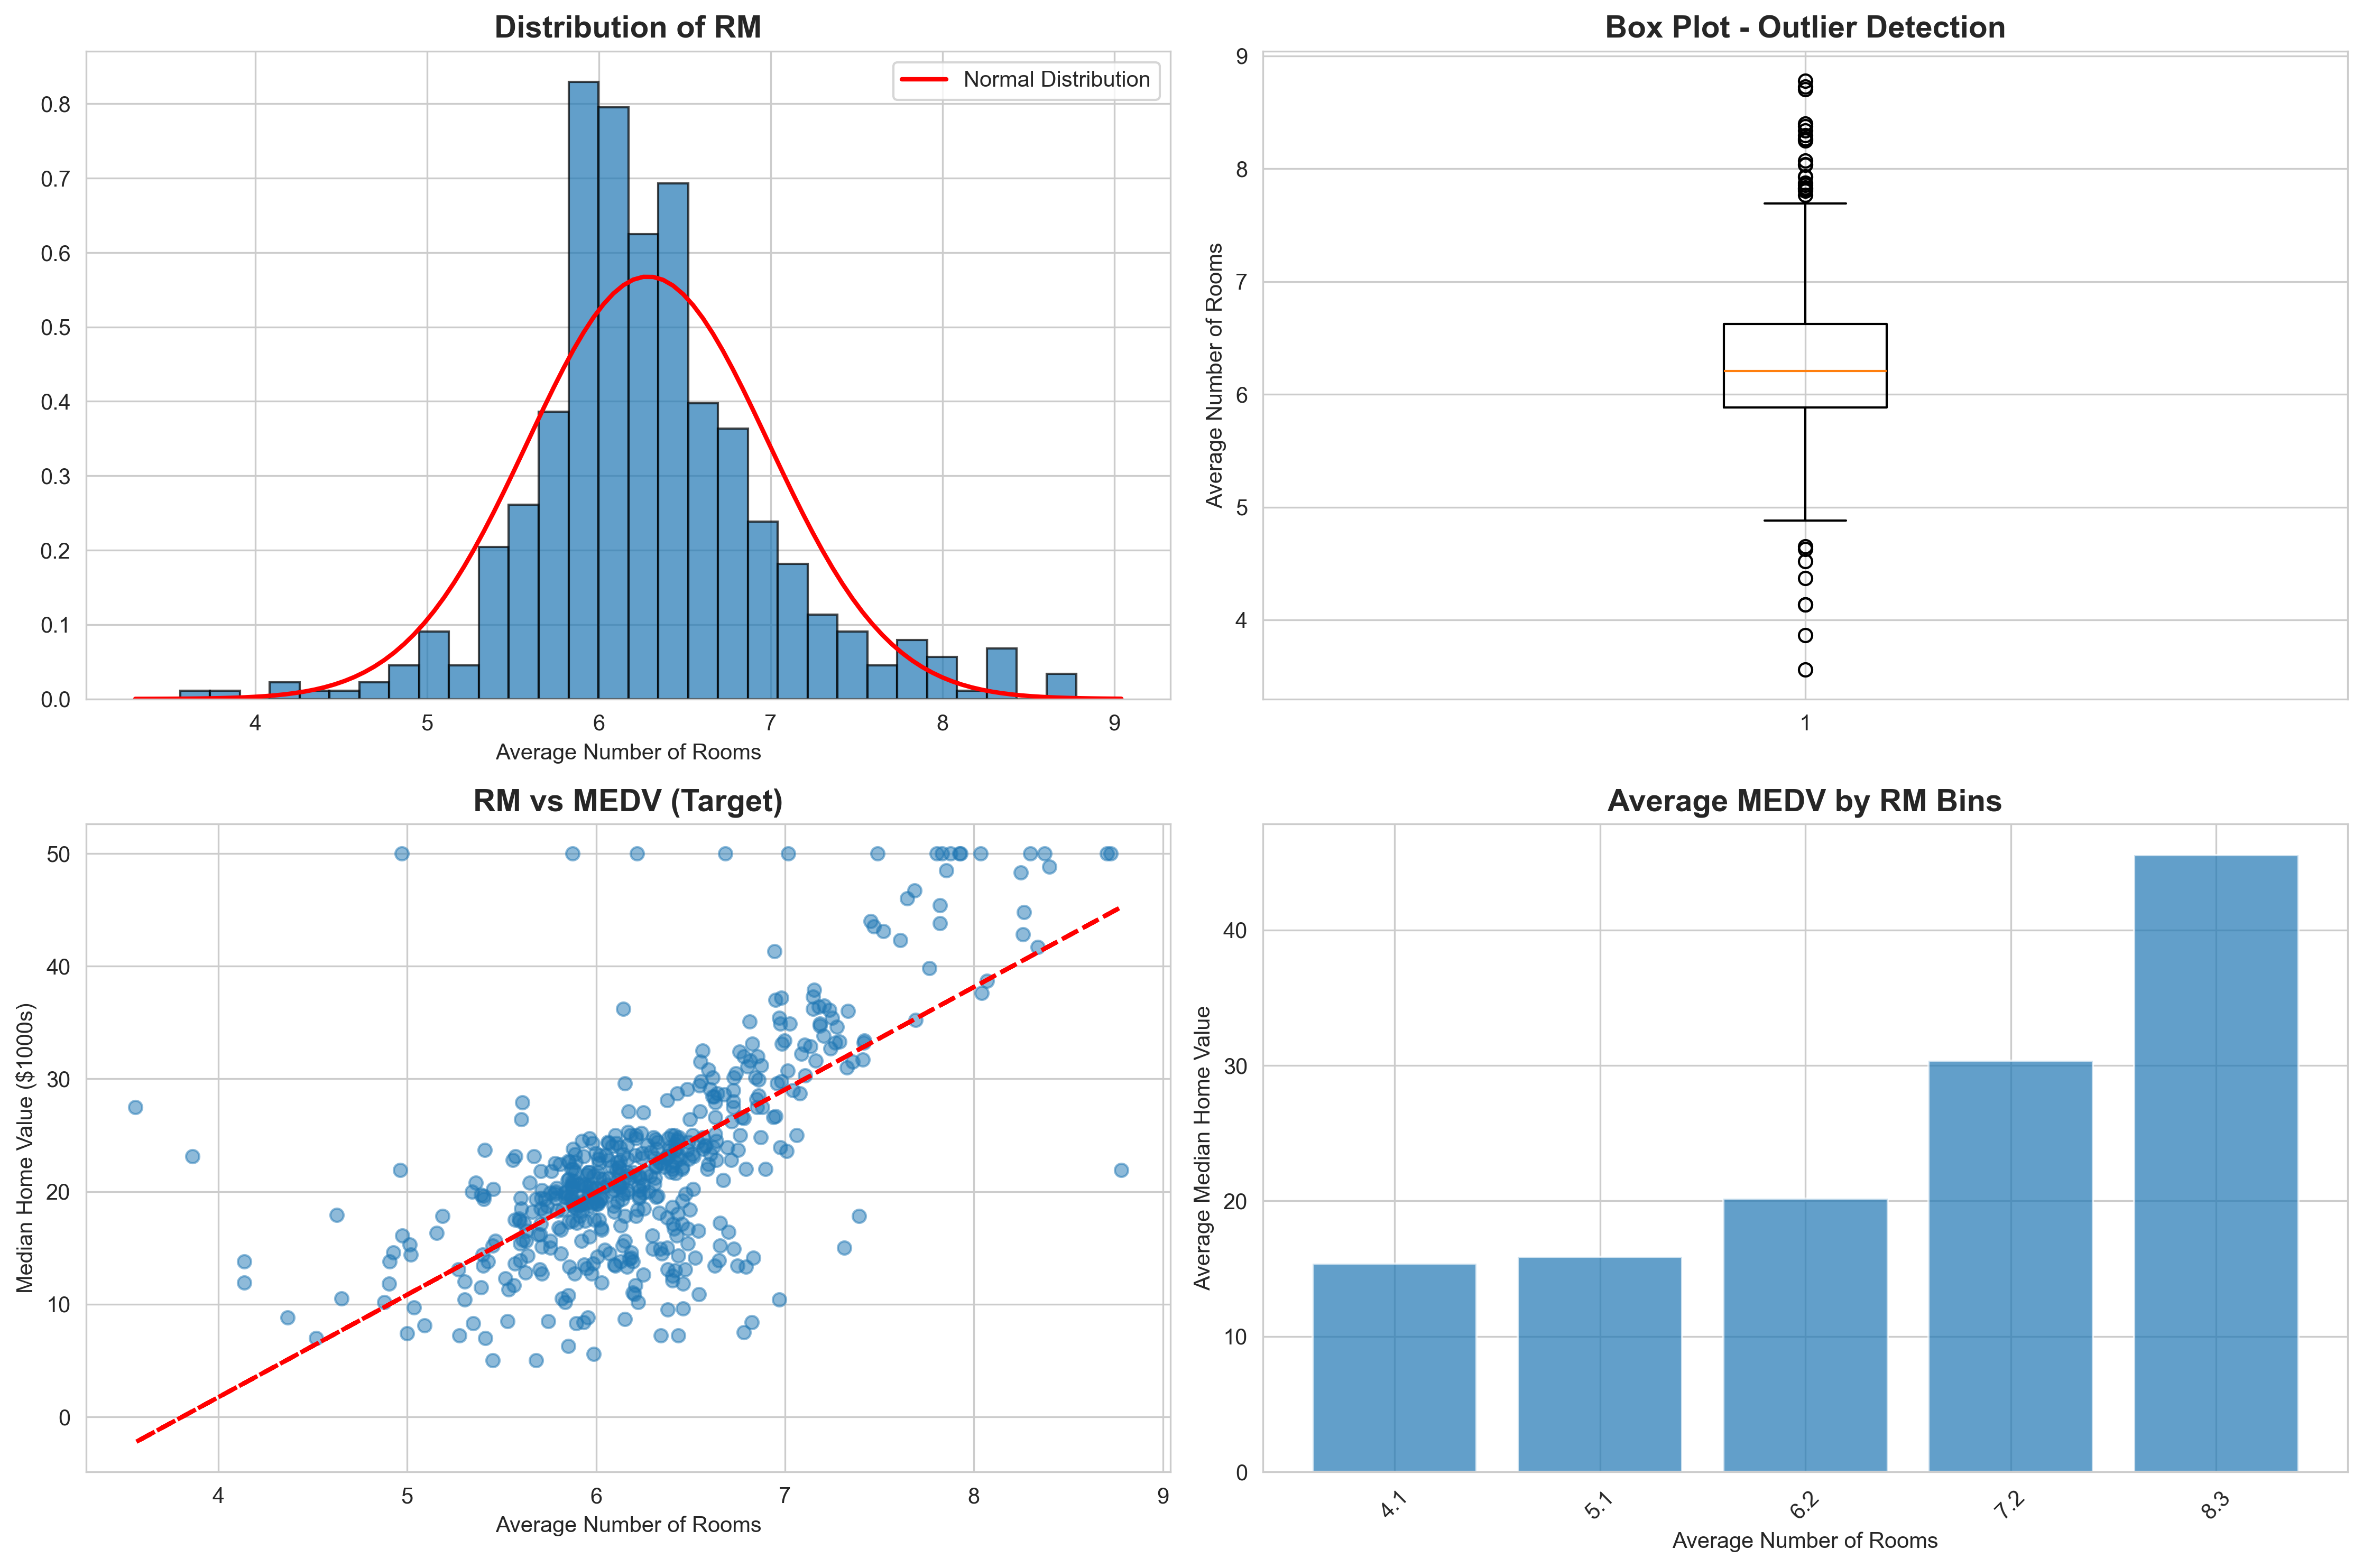
\includegraphics[width=0.85\linewidth]{images/rm_analysis.png}
    \caption{Subplot of Graphs Showing Correlation of RM to MEDV}
    \label{fig:rm_analysis}
\end{figure}

I created a graph for the distribution of RM (average number of rooms per dwelling),
a box plot to find outliers, a scatterplot with the target MEDV, and a binned analysis just to see if there were any other patterns available (which there were!).

But, continuing this method with other features resulted in less exciting results.

\begin{lstlisting}
    RAD: Correlation with MEDV (target): -0.382
    TAX: Correlation with MEDV (target): -0.469
    INDUS: Correlation with MEDV (target): -0.484
    CRIM: Correlation with MEDV (target): -0.388
    ZN: Correlation with MEDV (target): 0.360
    DIS: Correlation with MEDV (target): 0.250
    B-1000(Bk-0.63)^2: Correlation with MEDV (target): 0.333
\end{lstlisting}

Really not that exciting of findings! The best we could find in that whole debacle was the inverse correlation \lstinline{INDUS} had with the target. Which really isn't that helpful anyways.

But then I struck gold\dots

\begin{lstlisting}
LSTAT: Correlation with MEDV (target): -0.738
\end{lstlisting}

Wow! A nearly 74\% inverse correlation with the target. Now we are getting somewhere. Let's visualize that relation as well.

\begin{figure}[H]
    \centering
    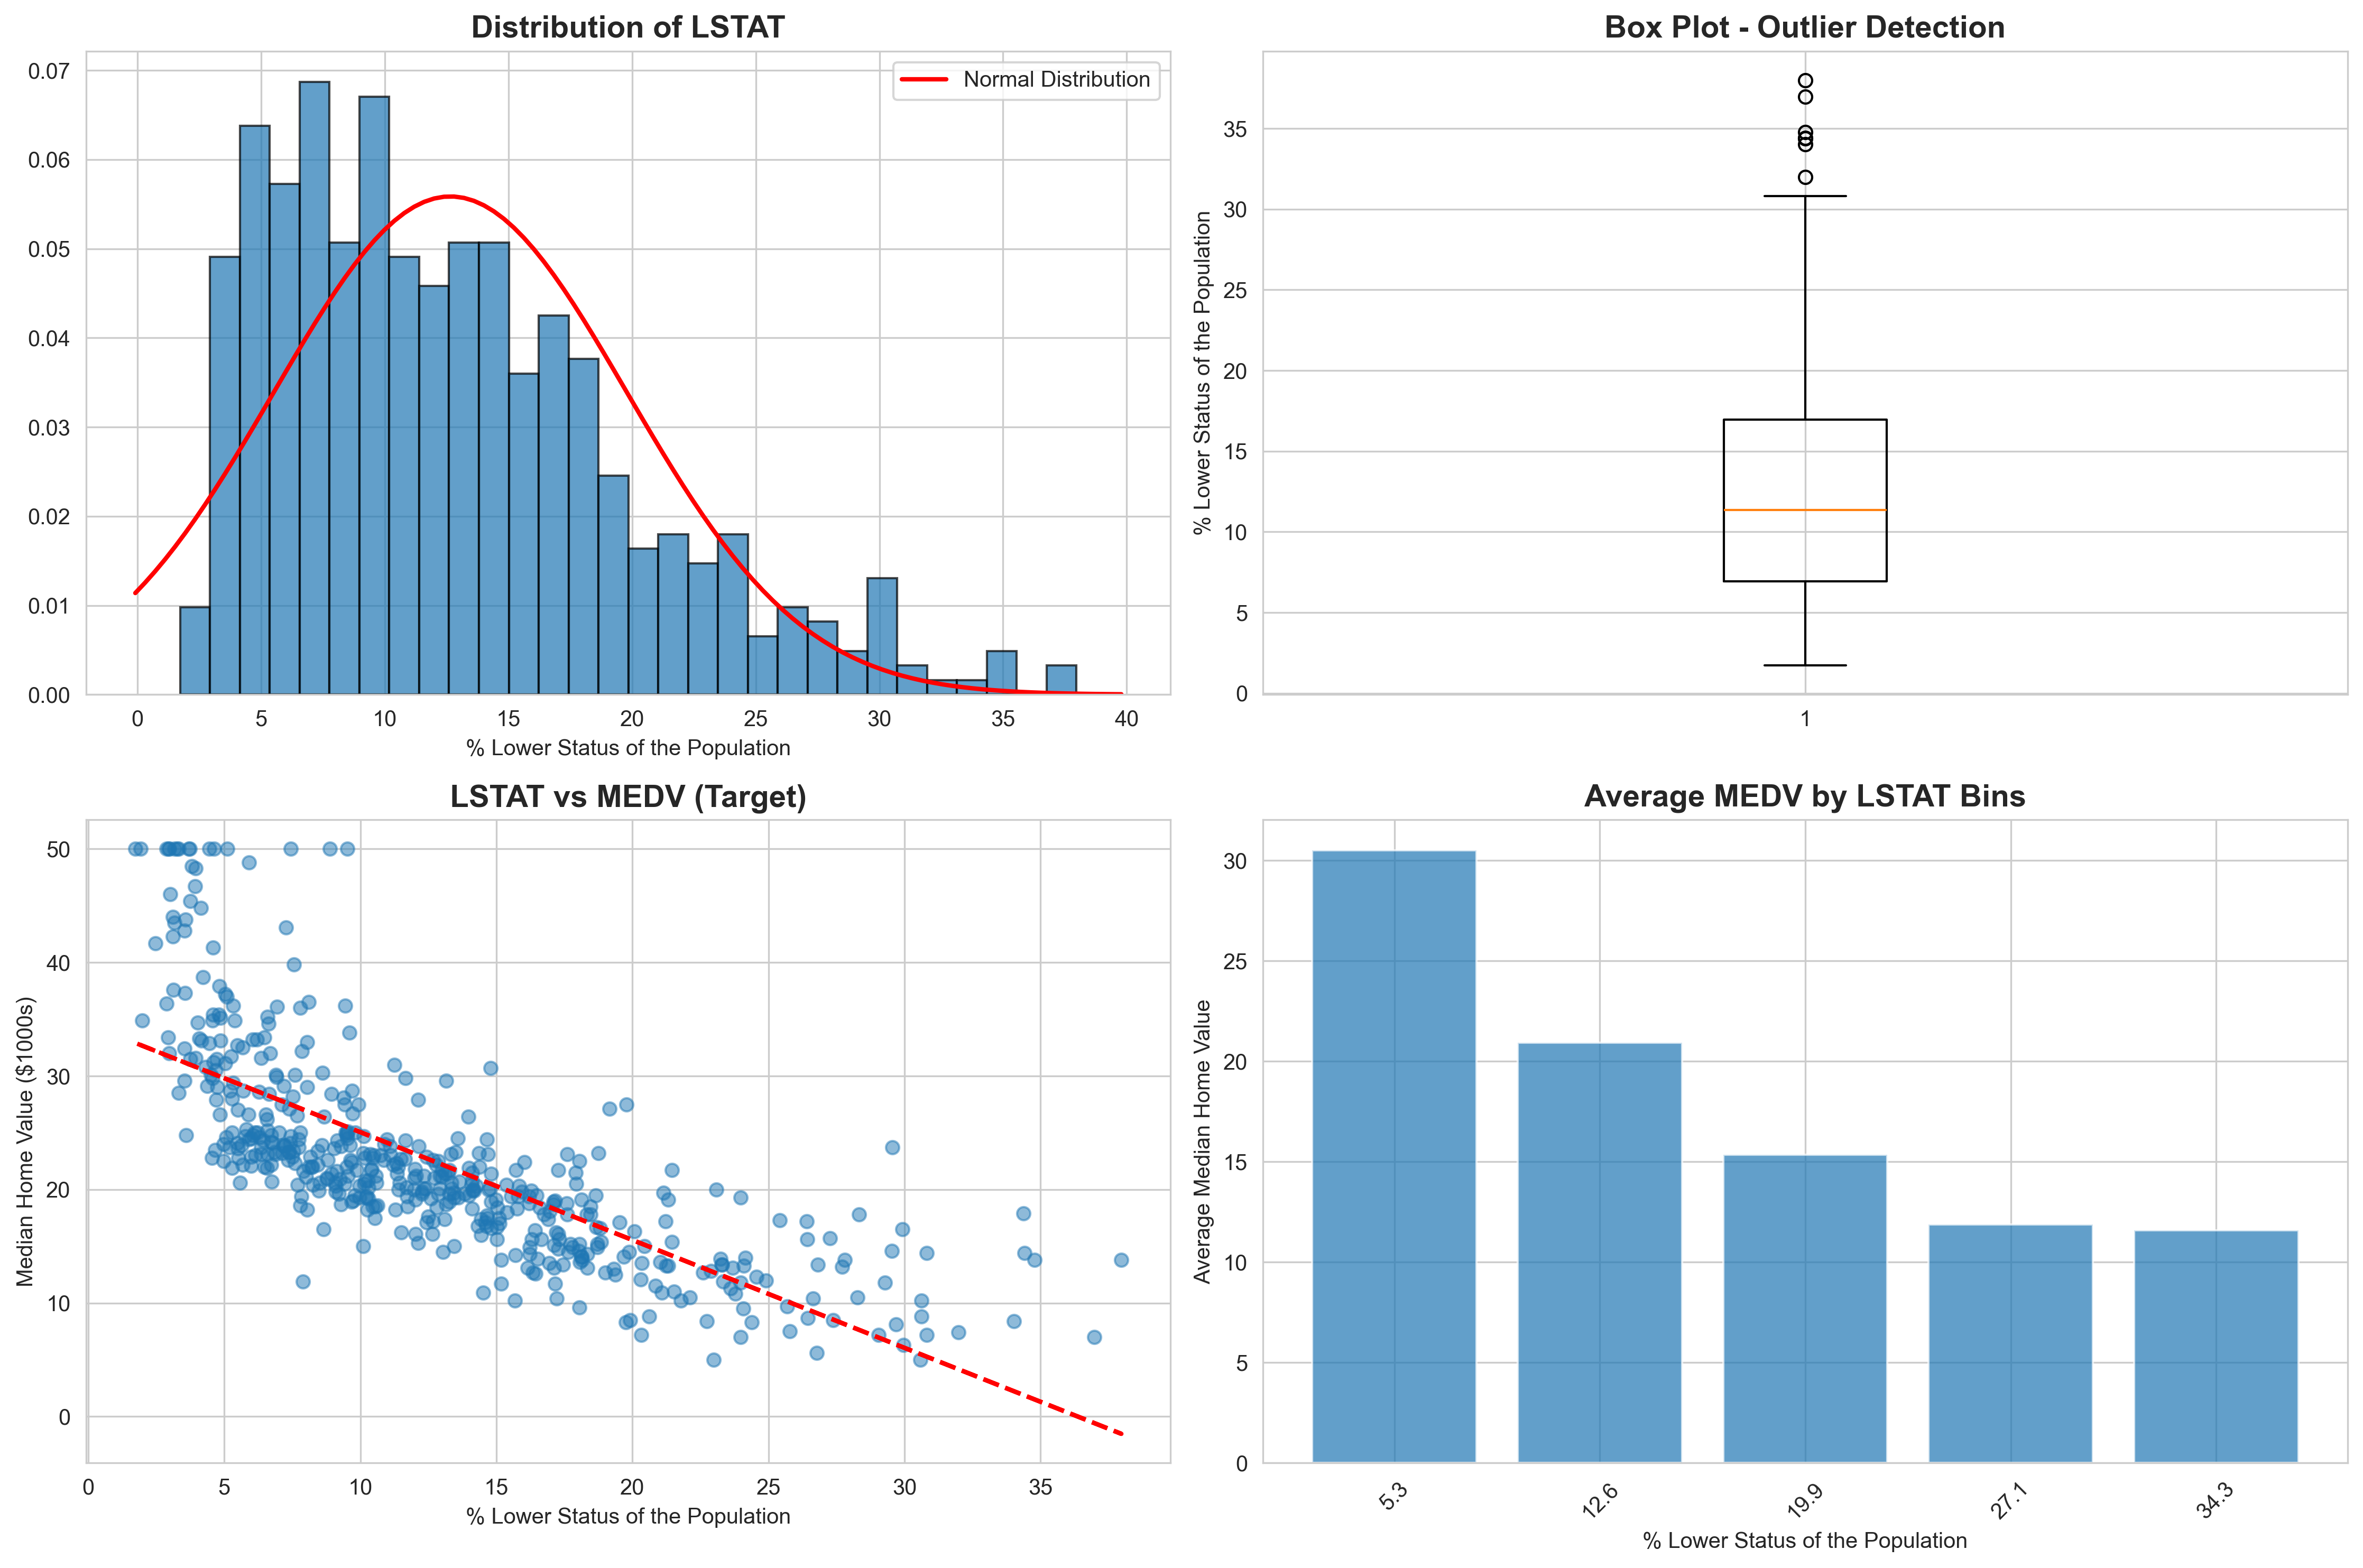
\includegraphics[width=0.85\linewidth]{images/lstat_analysis.png}
    \caption{Subplot of Graphs Showing Correlation of LSTAT to MEDV}
    \label{fig:lstat_analysis}
\end{figure}

However, I remembered from a machine learning course that I took that there was a method to find the best features automatically. So I did that.

\subsection{Exploratory Analysis}

The exploratory analysis showed that the top 5 features are \lstinline{LSTAT, RM, PTRATIO, TAX} and \lstinline{INDUS}. 
Generating a correlation matrix, feature correlation with target, target variable distribution, and the top 3 correlated features vs. \lstinline{MEDV} looks like

\begin{figure}[H]
    \centering
    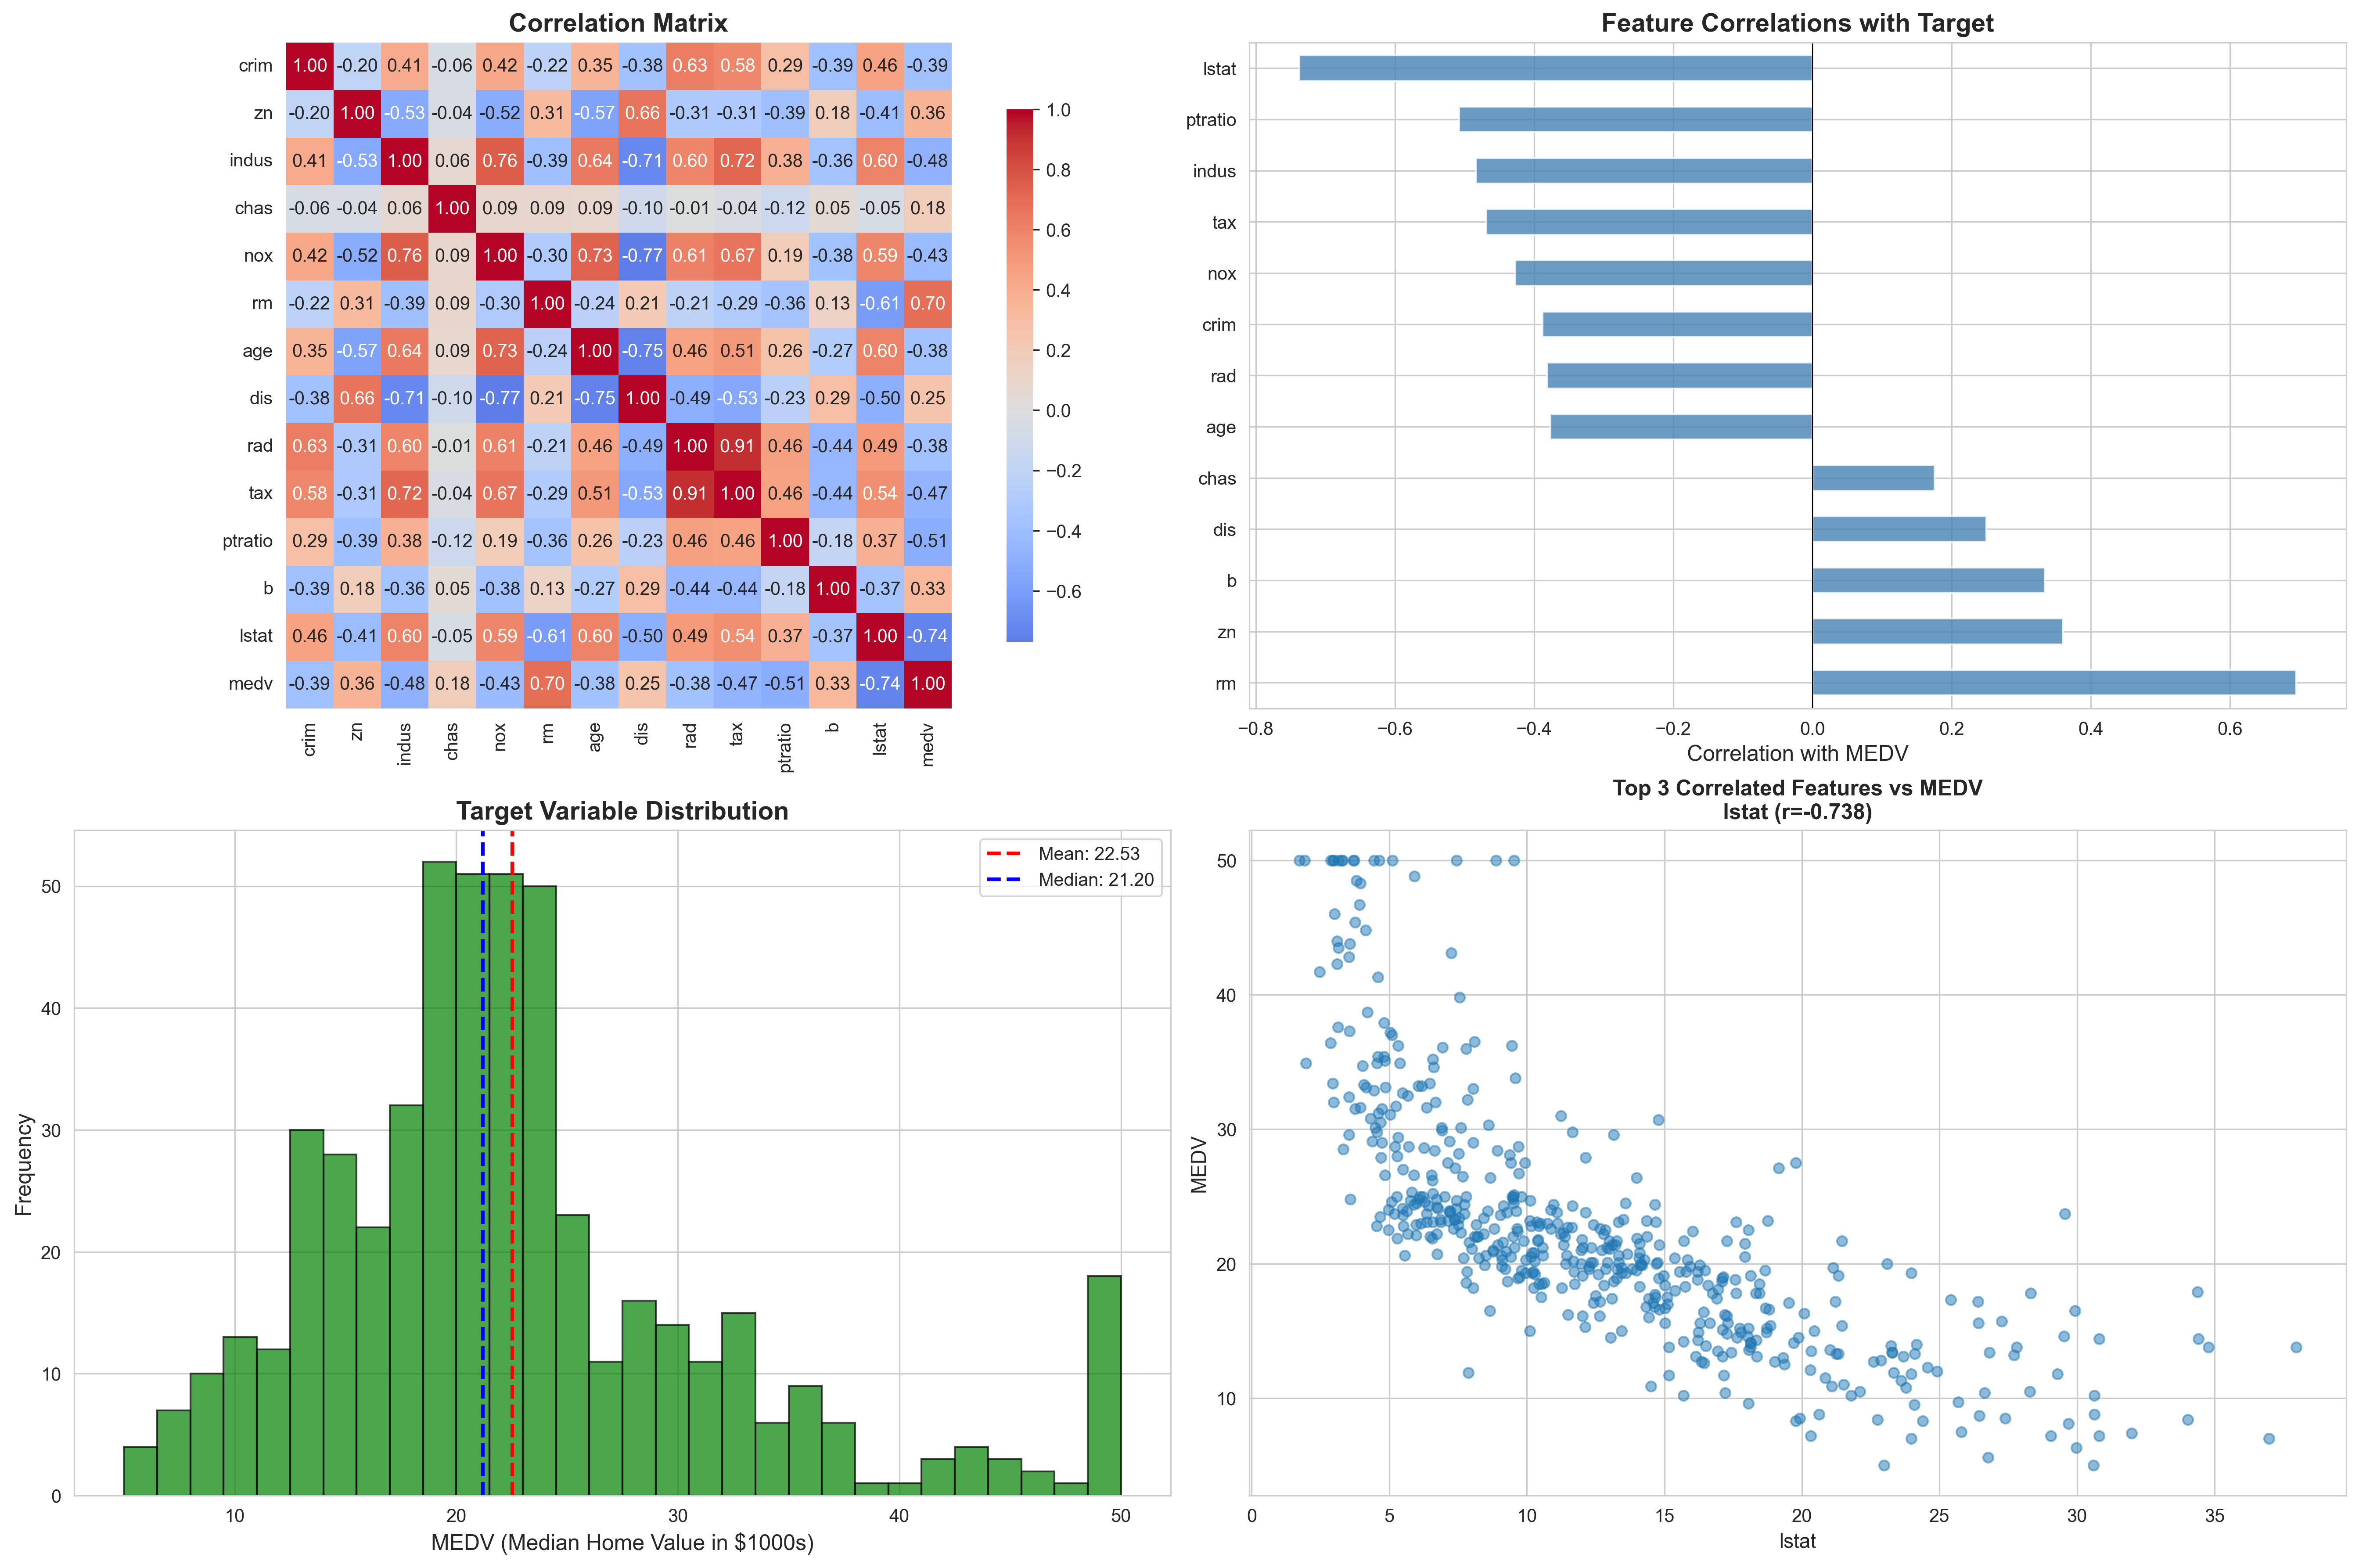
\includegraphics[width=0.85\linewidth]{images/01_exploratory_analysis.png}
    \caption{Subplot of Graphs Showing Analysis of Features}
    \label{fig:exploratoryanalysis}
\end{figure}

Afterwards I checked the multicolinearity between features with a high correlation and found 

\begin{lstlisting}
    Multicollinearity Check (Features with |correlation| > 0.7):
  indus <-> nox: 0.764
  indus <-> dis: -0.708
  indus <-> tax: 0.721
  nox <-> age: 0.731
  nox <-> dis: -0.769
  age <-> dis: -0.748
  rad <-> tax: 0.910

Train set size: 404, Test set size: 102
\end{lstlisting}

which shows that RAD and TAX, AGE and DIS, and NOX and DIS have the highest correlations among the outputs. With this understood, we can do linear regression on a subset of features chosen by the analysis.
The feature selection analysis tested subsets from 1 to 13 features. Cross-validation revealed that using all 13 features produced the highest R² score of 0.6688. This suggests that even weakly correlated features (like ZN with r=0.36) contribute meaningful information when combined in the linear model. The feature selection curve (Figure \ref{fig:linearregression}, top-left) shows that performance plateaus after 8-10 features, with marginal gains from additional features.

\subsection{Linear Regression}

After applying linear regression, we get these output plots and we are mainly interested in the bottom right graph.

\begin{figure}[H]
    \centering
    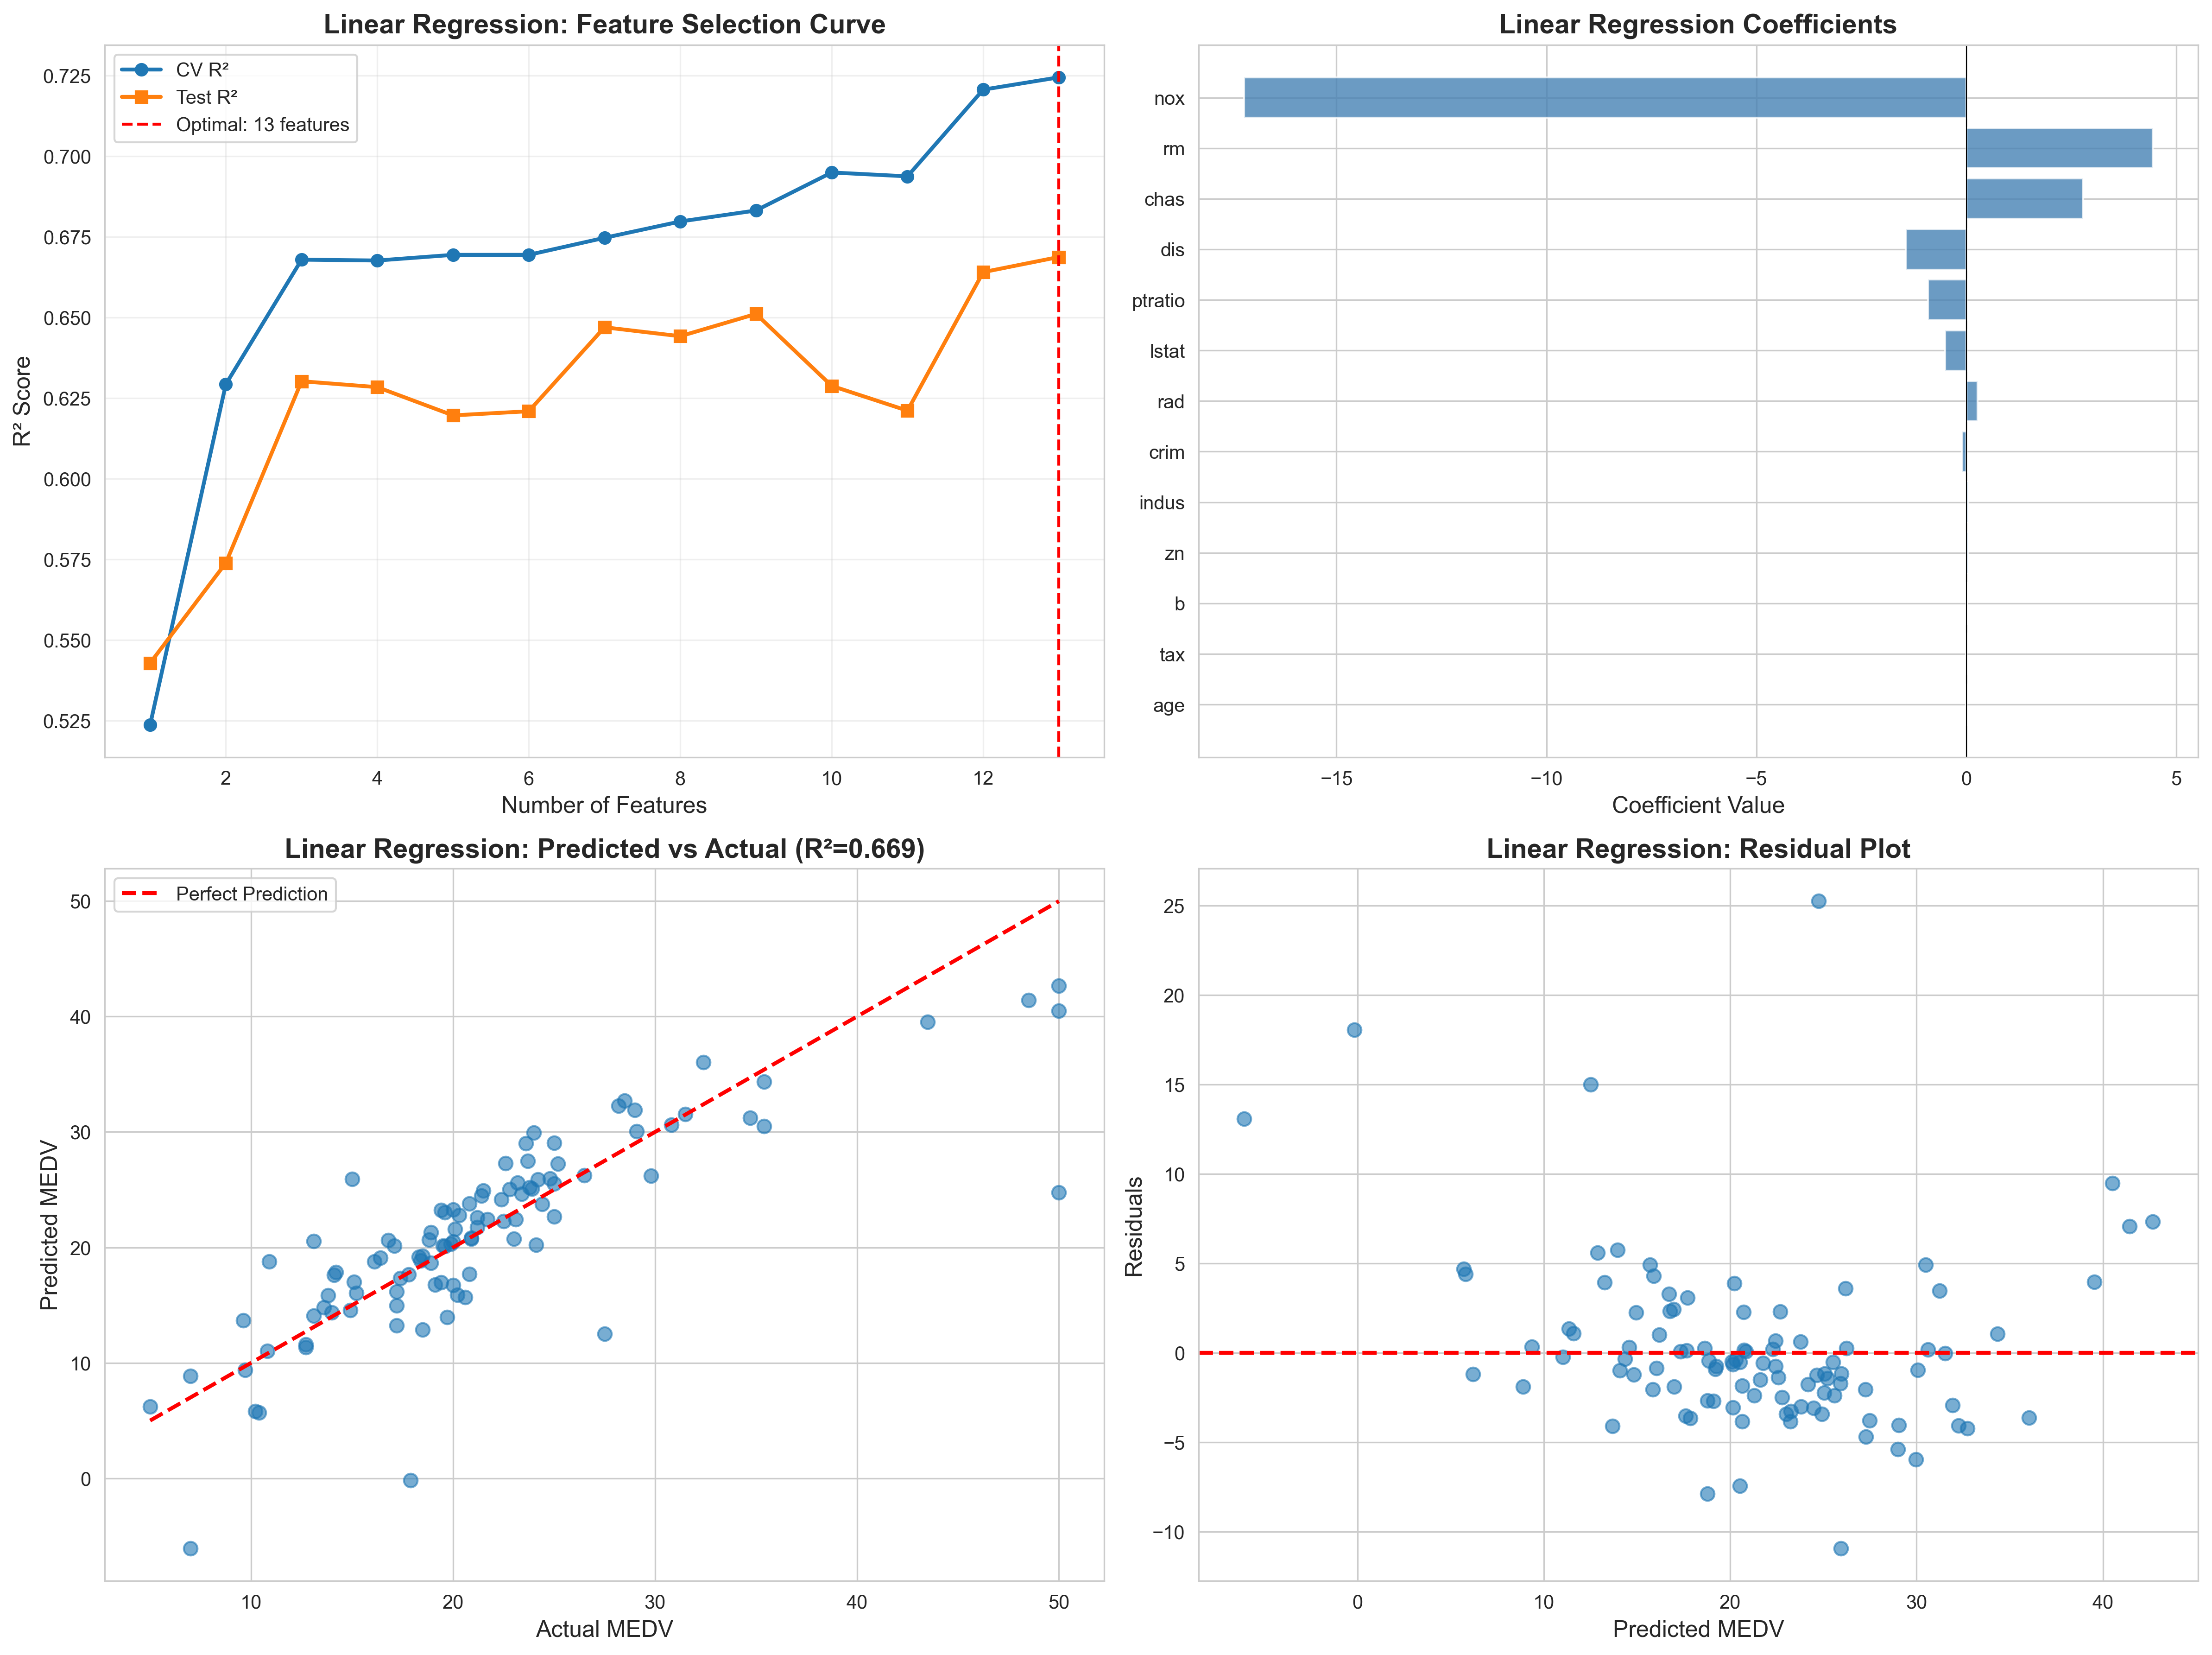
\includegraphics[width=0.85\linewidth]{images/02_linear_regression.png}
    \caption{Subplot of Graphs Showing Linear Regression}
    \label{fig:linearregression}
\end{figure}

\subsection{Ridge Regression}

Now, Ridge Regression (and Lasso) do not need the feature selection because they'll do it on there own! 
After creating a scaler object from sklearn, I found the optimal alpha via cross-validation to use, and then found the $R^2$ value.

\begin{figure}[H]
    \centering
    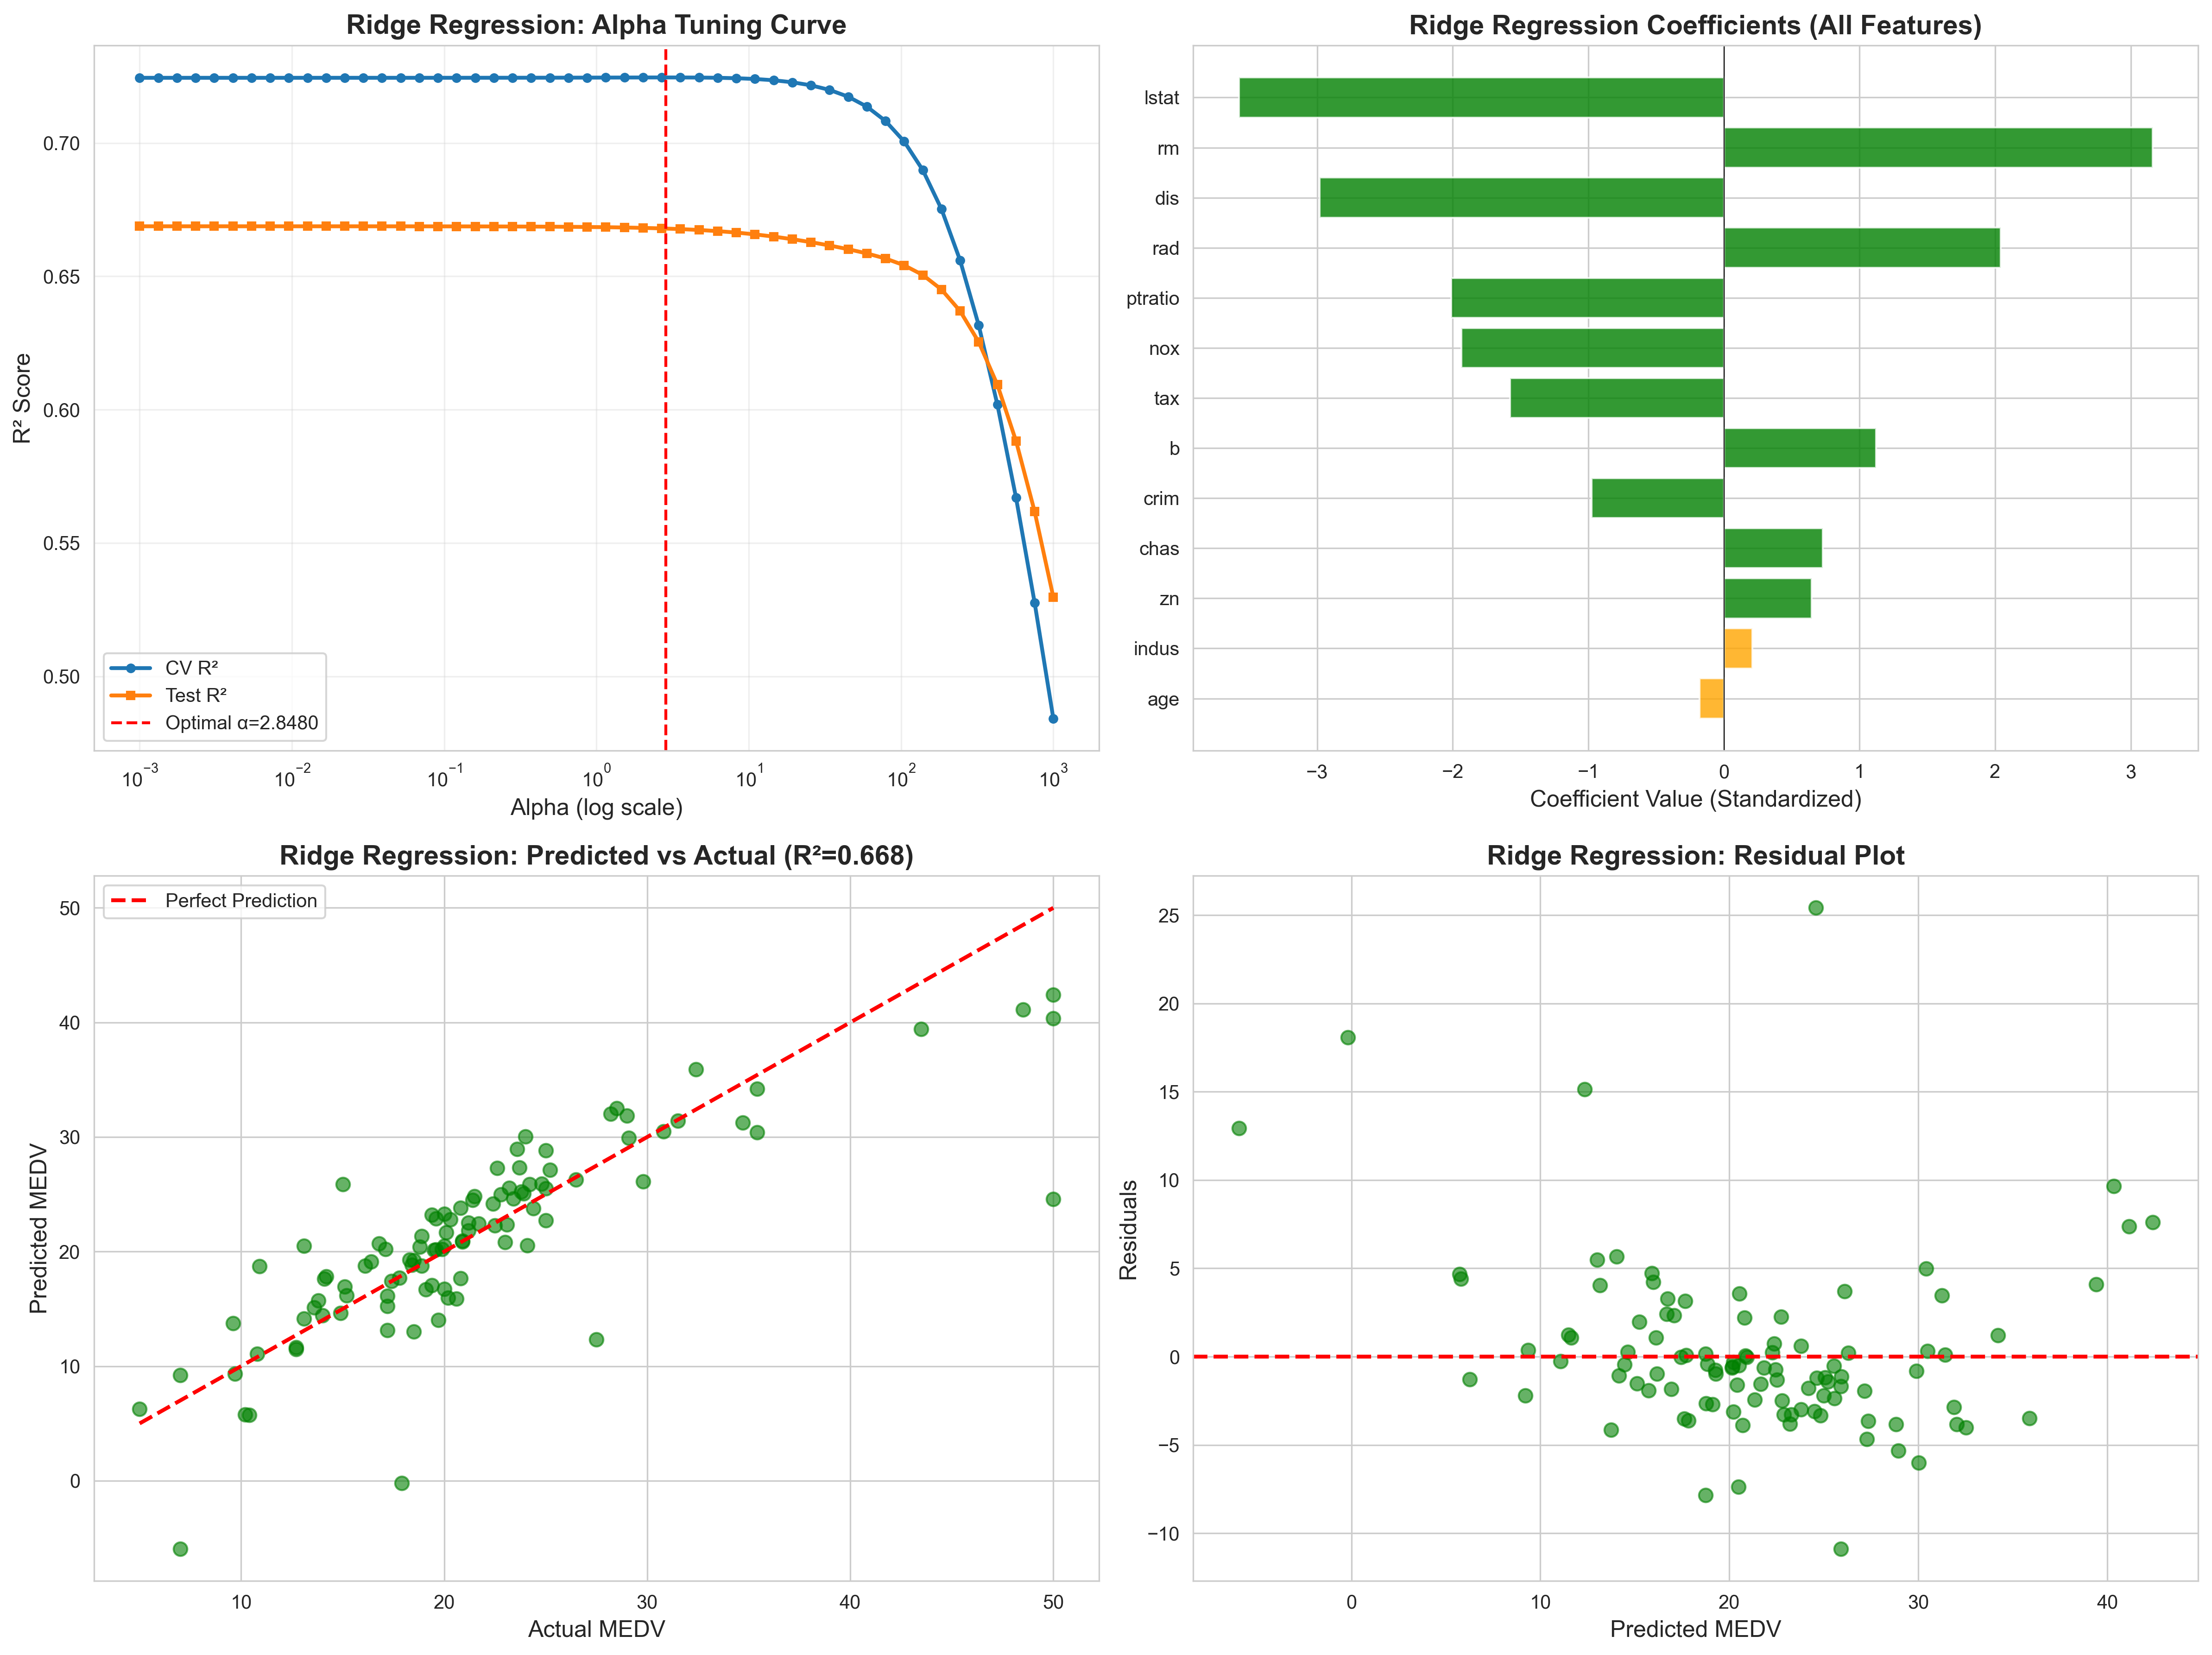
\includegraphics[width=0.85\linewidth]{images/03_ridge_regression.png}
    \caption{Subplot of Graphs Showing Ridge Regression}
    \label{fig:ridgeregression}
\end{figure}

\subsection{Lasso}

Finally, we have Lasso. Again, this method doesn't need feature selection. So, running lasso after finding the optimal alpha, this is what was produced.
Figure \ref{fig:lasso} shows Lasso's performance. The bottom-right subplot reveals that Lasso selected the same 9 features as Linear Regression initially identified as most important, validating our manual feature selection approach. Notably, Lasso eliminated AGE, INDUS, CHAS, and ZN, which were among the weakest predictors.

\begin{figure}[H]
    \centering
    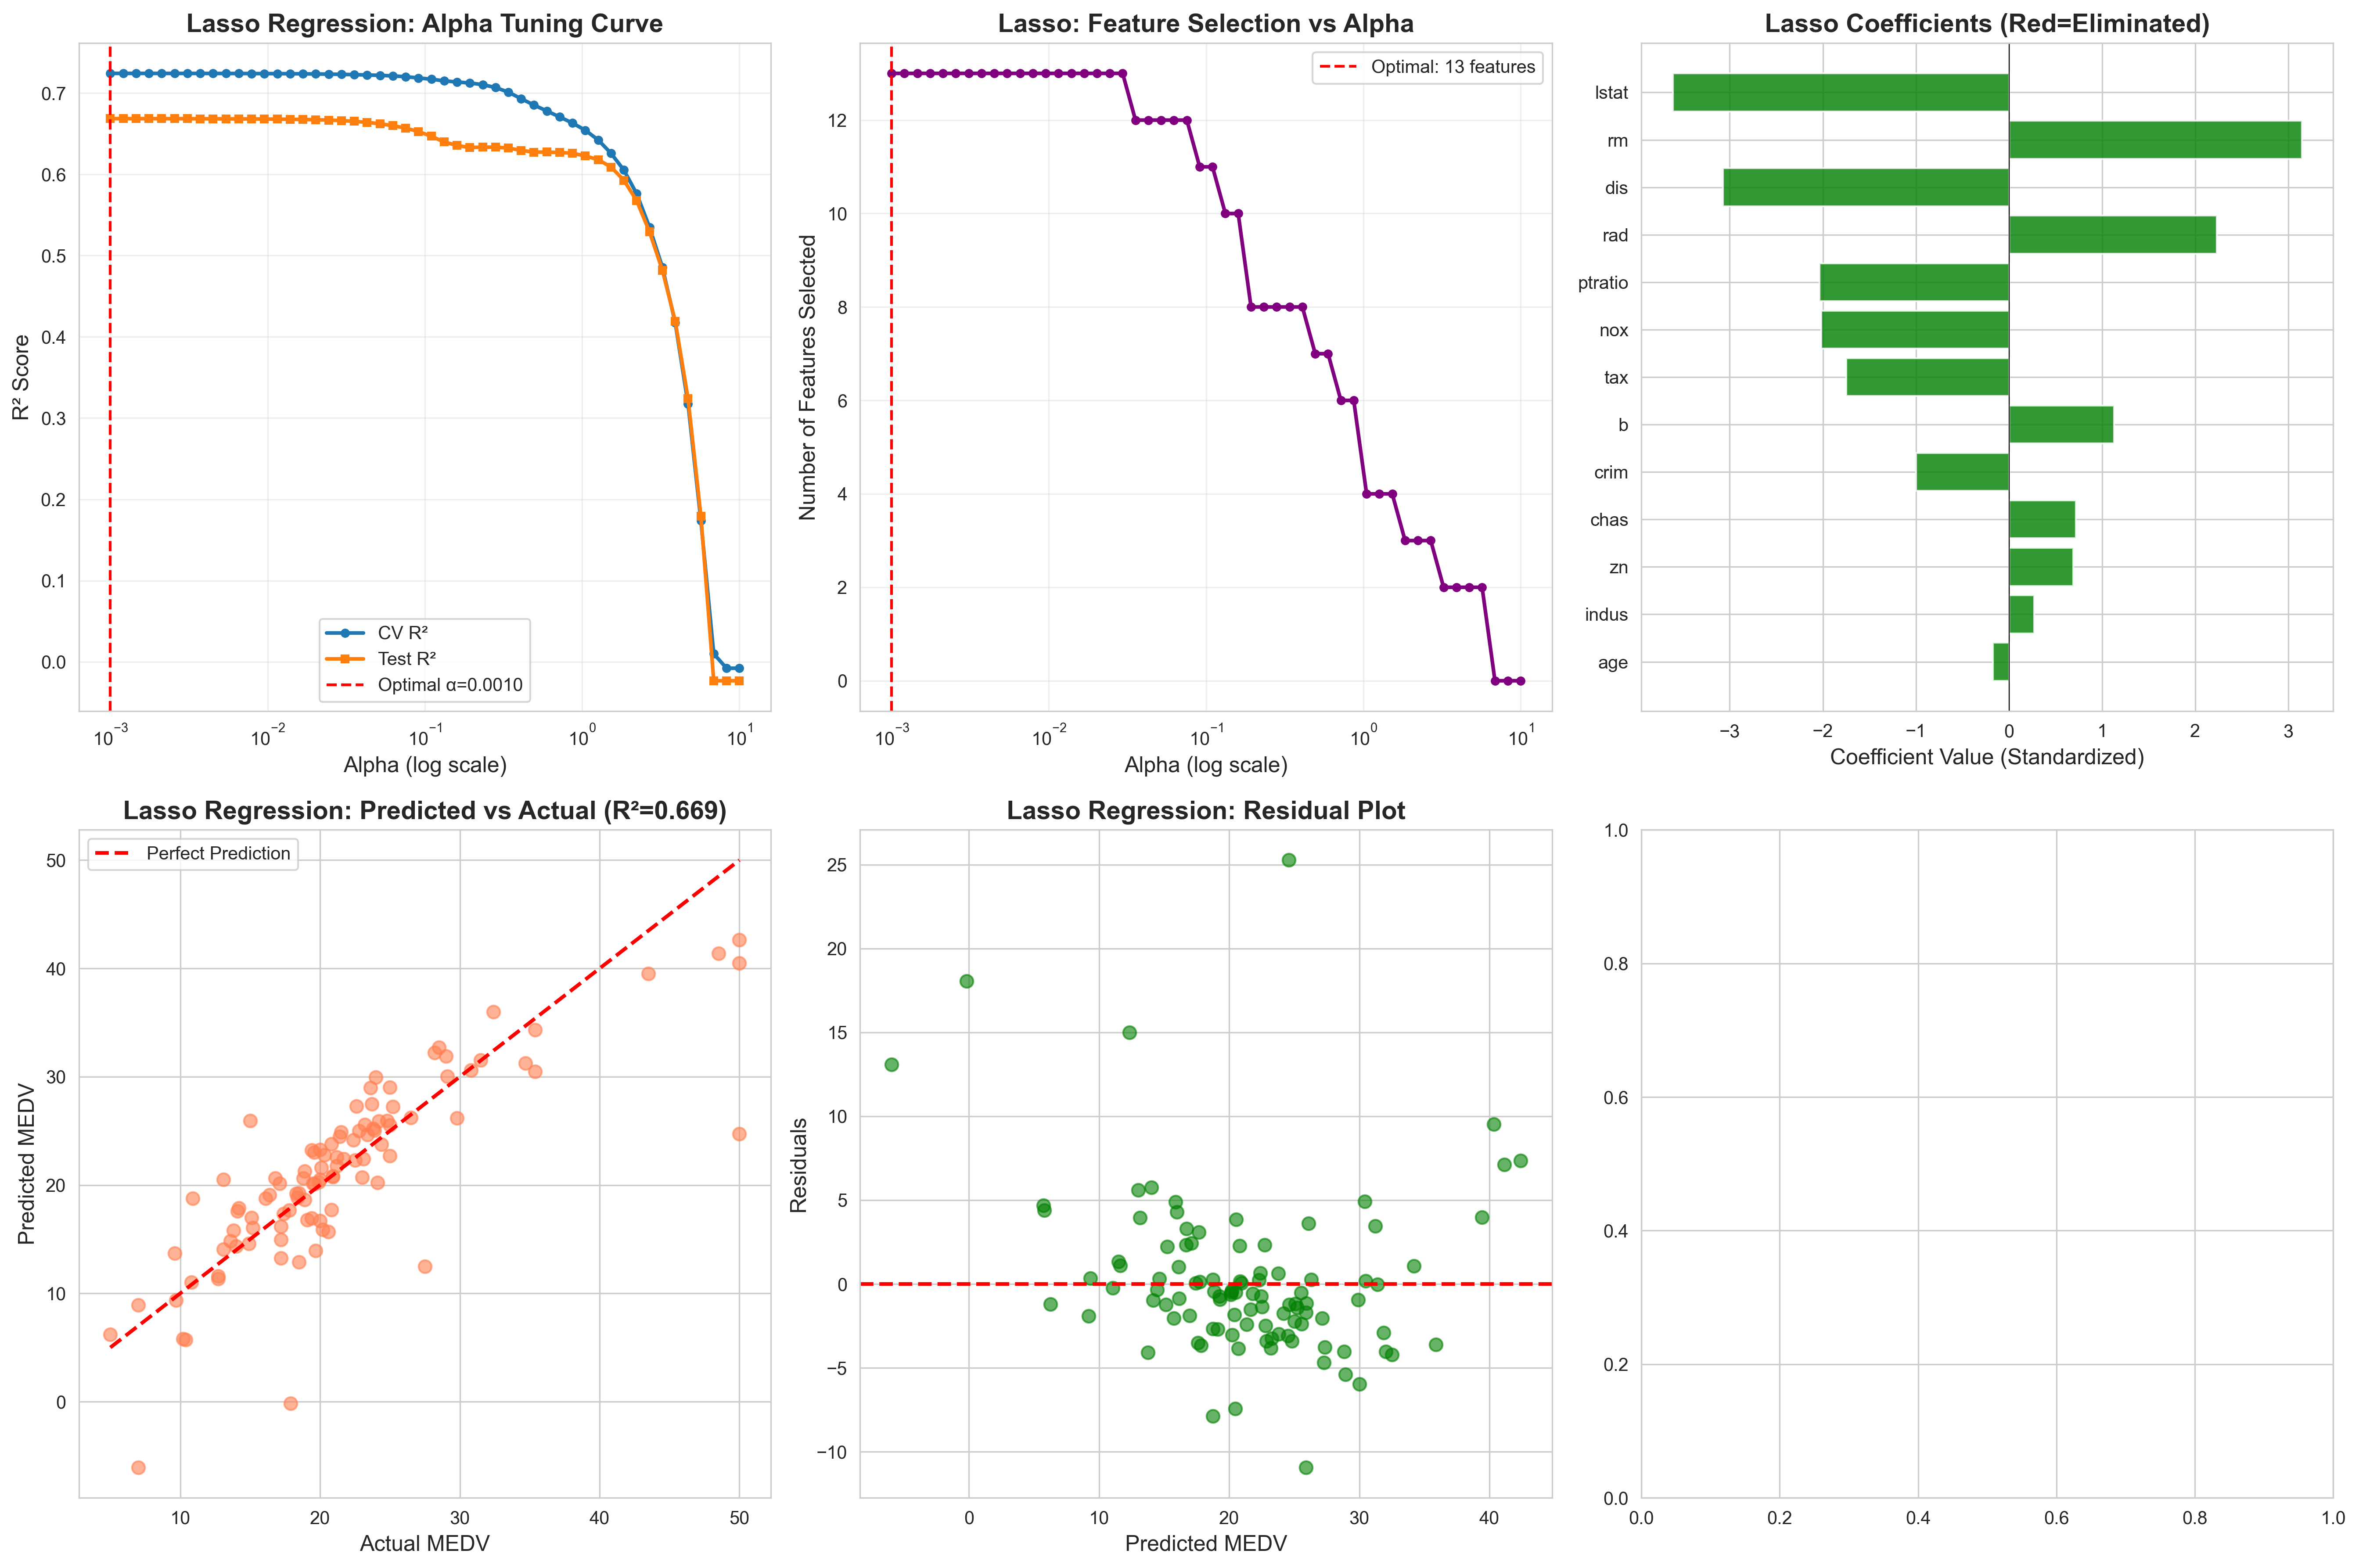
\includegraphics[width=0.85\linewidth]{images/04_lasso_regression.png}
    \caption{Subplot of Graphs Showing Lasso}
    \label{fig:lasso}
\end{figure}

\subsection{Comparison and Conclusions}

\begin{table}[H]
\centering
\begin{tabular}{|l|c|c|c|c|}
\hline
\textbf{Method} & \textbf{Features Used} & \textbf{Test R²} & \textbf{Test RMSE} & \textbf{Test MAE} \\
\hline
Linear Regression & 13 & 0.6688 & 4.9286 & 3.1891 \\
Ridge Regression & 13 & 0.6679 & 4.9349 & 3.1815 \\
Lasso Regression & 13 & 0.6687 & 4.9289 & 3.1882 \\
\hline
\end{tabular}
\caption{Comparison of Regression Methods on Boston Housing Dataset}
\label{tab:comparison}
\end{table}

\textbf{Performance Analysis:}

Looking at the results, all three methods performed almost identically! The test R² scores 
ranged from 0.6679 to 0.6688, meaning each model explains about 67\% of the variance in home prices. 
The RMSE values are basically the same too (around 4.93-4.95), which means our predictions 
are off by roughly \$4,900 on average.

\textbf{Feature Selection Results:}

Here's where things got interesting - all three methods ended up using all 13 features:

\begin{itemize}
    \item \textbf{Linear Regression}: The cross-validation kept adding features and 
    performance kept improving, maxing out at R² = 0.7244 when using all 13. Even the 
    weaker features like CHAS (F-score = 15.16) contributed something useful.
    
    \item \textbf{Ridge Regression}: With $\alpha = 2.848$, Ridge kept all the features 
    but shrunk their coefficients. You can see this clearly with NOX, which went from 
    -17.20 in Linear Regression down to -1.94 in Ridge - that's the regularization at work!
    
    \item \textbf{Lasso Regression}: The optimal $\alpha = 0.001$ was tiny, so Lasso 
    barely regularized at all and didn't eliminate any features. Turns out that for 
    this dataset, all the features are actually helpful and cutting any of them would 
    hurt performance.
\end{itemize}

\textbf{Handling Multicollinearity:}

Remember that multicollinearity we found earlier? (RAD-TAX at 0.91, NOX-DIS at -0.77) 
Well, the regularization methods handled it pretty well:

\begin{itemize}
    \item Linear Regression had some wild coefficient values (NOX = -17.20!), which is 
    a red flag for multicollinearity issues
    \item Ridge smoothed everything out and gave more reasonable, stable coefficients
    \item Both Ridge and Lasso ended up with similar standardized coefficients, suggesting 
    they both found good solutions to the multicollinearity problem
\end{itemize}

\textbf{Overfitting Analysis:}

\begin{table}[H]
\centering
\begin{tabular}{|l|c|c|c|}
\hline
\textbf{Method} & \textbf{Train R²} & \textbf{Test R²} & \textbf{Overfit Gap} \\
\hline
Linear Regression & 0.7509 & 0.6688 & 0.0821 \\
Ridge Regression & 0.7508 & 0.6679 & 0.0829 \\
Lasso Regression & 0.7509 & 0.6687 & 0.0822 \\
\hline
\end{tabular}
\caption{Overfitting Analysis (Train R² - Test R²)}
\label{tab:overfit}
\end{table}

All three models showed about the same amount of overfitting (gap of around 0.082), 
which is actually not bad at all. The fact that Ridge and Lasso didn't reduce overfitting 
much compared to regular Linear Regression suggests our dataset is big enough (506 samples) 
for the 13 features we're using.

\textbf{Most Important Features:}

Looking at the coefficient magnitudes across all methods, the top 5 features that matter most are:

\begin{enumerate}
    \item \textbf{LSTAT} (lower status \%): The strongest predictor at -3.61
    \item \textbf{RM} (rooms): Close second at +3.15
    \item \textbf{DIS} (distance to employment): -3.07
    \item \textbf{RAD} (highway access): +2.23
    \item \textbf{PTRATIO} (pupil-teacher ratio): -2.04
\end{enumerate}

This matches perfectly with what we found in the exploratory analysis - LSTAT (-0.738 correlation) 
and RM (+0.695 correlation) were our stars from the beginning!

\textbf{Key Takeaways:}

\begin{itemize}
    \item Even with all that multicollinearity, every feature ended up being useful
    \item Lasso's tiny alpha (0.001) tells us that cutting features would actually 
    make things worse for this dataset
    \item Ridge's coefficient shrinkage really helped stabilize things - just look 
    at how NOX went from -17.20 to -1.94!
    \item The nearly identical performance across all three methods means this dataset 
    plays nice with linear models and doesn't need heavy regularization
\end{itemize}

\section{Code}

I think I got it working this time. Thank you TA's for your hard work. Please enjoy your week(end) :)
\begin{center}
    \Large{\href{https://colab.research.google.com/drive/1ZwY5hkh6zIxvTSQysjWt4UU_HUVPftSI?usp=sharing}{THE CODE}}
\end{center}

\end{document}